\subsection{Task 2}
\label{sec:task2results}


The main differences between the $k-\epsilon$ and $k-\omega$ models have been discussed in section \ref{sec:task2}. In this section, their results for this specific case will be examined and compared. Especially, the recirculation zone and the vicinity of the expansion of the pipe will be studied.\\

\noindent While the same sketches and geometry is used from Task 1, also, grid convergence is achieved at the same mesh sizes as before. The mesh that was sufficiently fine was found when the element size was set to $5*10^{-4}$ meters. An image of this mesh can be seen from Figure \ref{fig:task2mesh}. Also, to confirm the achievement of steady state conditions, the residuals have been plotted an shown in Figure \ref{fig:task2_residuals}.

\begin{figure}[H]
    \centering
    \begin{subfigure}{.45\textwidth}
    \centering
    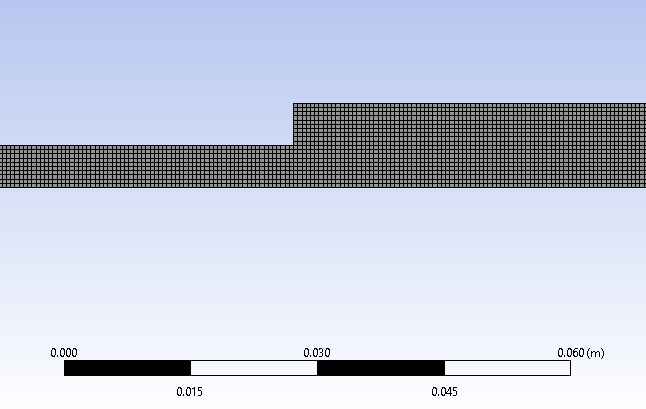
\includegraphics[width=.95\linewidth]{images/task2/task2-1/task2_mesh.png}
    \caption{Mesh for both models}
    \label{fig:task2mesh}
    \end{subfigure}
\hfill
\begin{subfigure}{.45\textwidth}
    \centering
    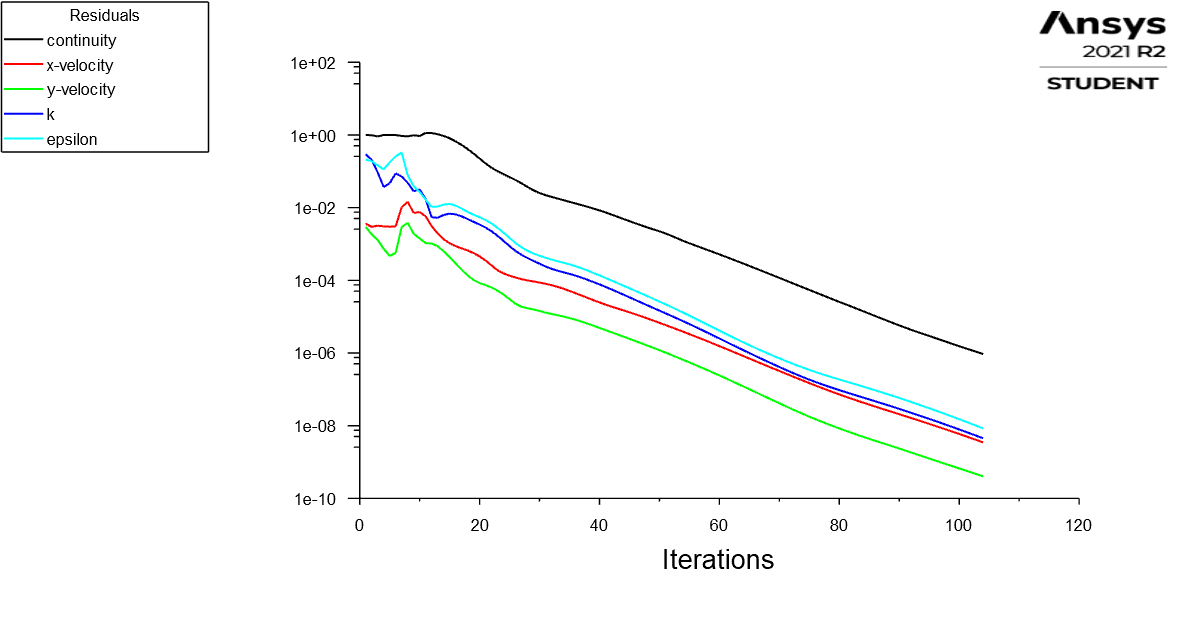
\includegraphics[width=.95\linewidth]{images/task2/task2-1/task2_1residuals.png}
    \caption{Residual plot for the models}
    \label{fig:task2_residuals}
\end{subfigure}
    
    \hfill
    \caption{Residuals and Mesh Sizes}
\end{figure}

\noindent Following this validation of the results. Also, the inlet and outlet fluxes have been compared and it was found that their difference was in the order of $10^{-9}$. Therefore, since we have shown that our simulation is seemingly meaningful, now I will be continuing with the comparisons of the models, starting with the velocity profiles.\\

\subsubsection{Comparison of the Velocity Profiles}

\noindent As can be seen from Figure \ref{fig:axial_task2}, while the main behavior is quite similar, there are deviations between the axial velocity profiles along the centerline. Specifically, there is a sudden and steep decrease in velocity after the expansion in both cases, however, this steep decrease is more delayed in the $k-\omega$. This feature clearly indicates a bigger recirculation zone and hints a longer reattachment length for the $k-\omega$ model. Besides this, the profiles are quite similar.\\


\noindent After this, velocity profiles from various cross sections have been gathered to be compared. The specific locations of those cross sections are shown with yellow lines in Figure \ref{fig:task2cross}. Particularly, these cross sections are taken from those that are inside or in the vicinity of the recirculation zone.\\

\begin{figure}[H]
    \centering
    \begin{subfigure}{.45\textwidth}
    \centering
    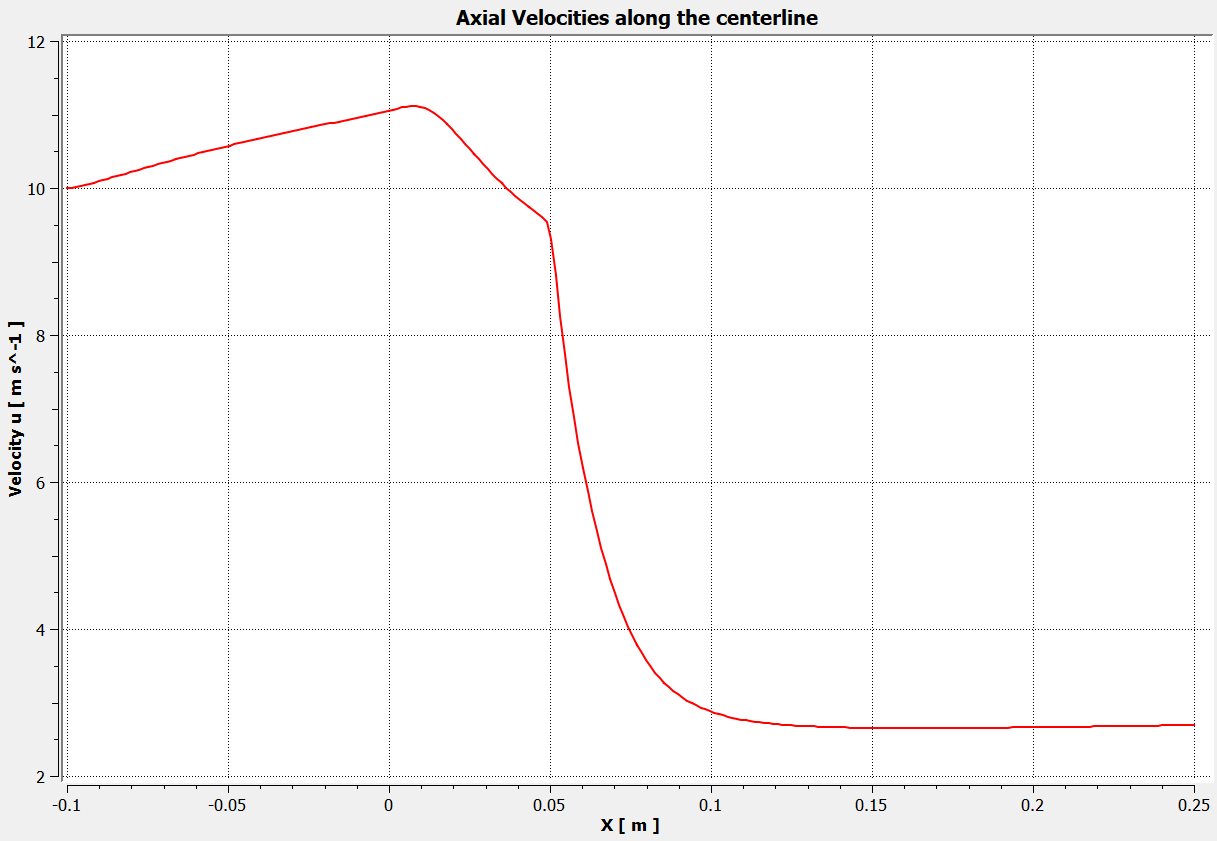
\includegraphics[width=.9\linewidth]{images/task2/task2-1/axial.png}
    \caption{Axial velocity profile of $k-\epsilon$ model}
    \label{fig:task2mesh}
    \end{subfigure}
    ~
\begin{subfigure}{.45\textwidth}
    \centering
    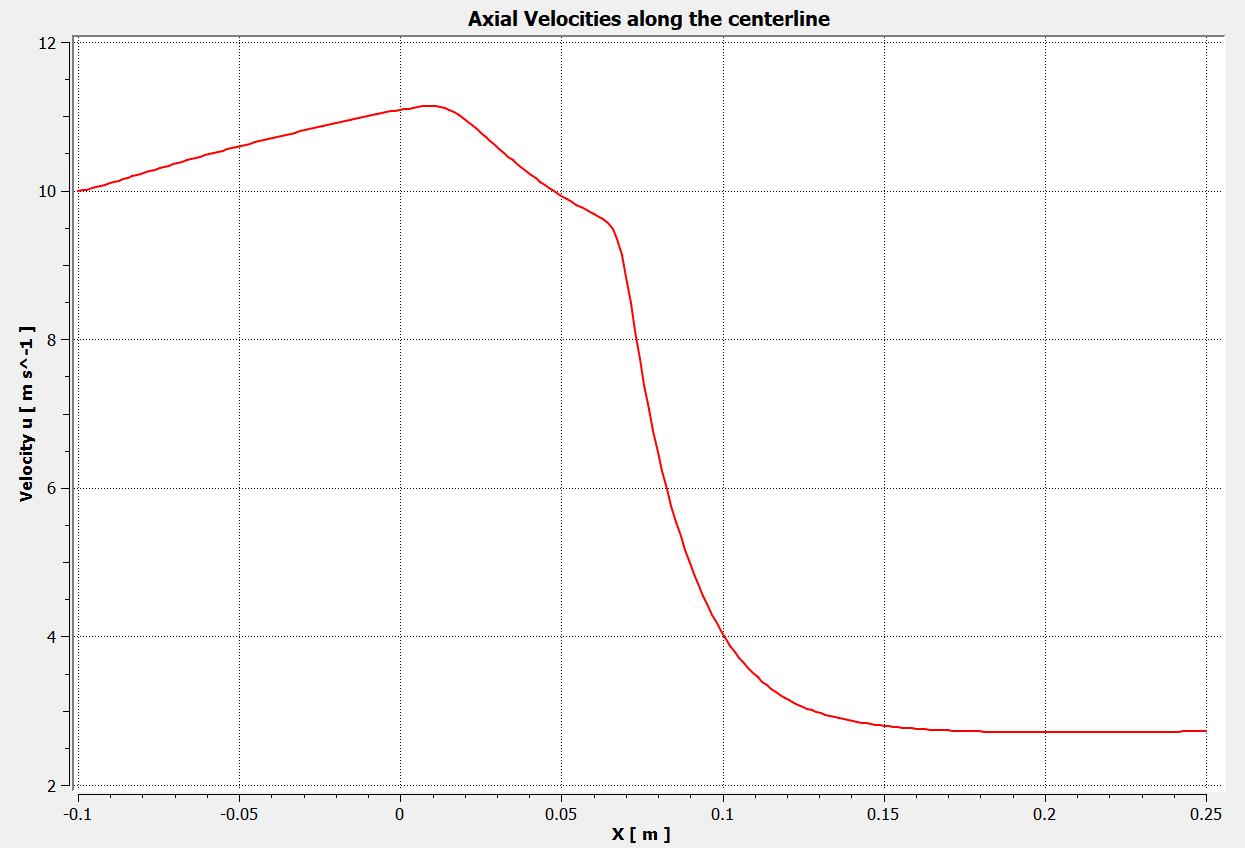
\includegraphics[width=.9\linewidth]{images/task2/task2-2/axials.png}
    \caption{Axial velocity profile of $k-\omega$ model}
    \label{fig:task2_residuals}
\end{subfigure}
    \caption{Axial velocity profiles}
    \label{fig:axial_task2}
\end{figure}


\noindent Further examination of the velocity profiles from different cross sections are shown comparatively on Figures \ref{fig:task2prof1} and \ref{fig:task2prof2}. On these plots, the discrepancies between the models are less apparent, especially in the vicinity of expansion. However, when looked at the cross sections from $x=20, 40, 60$ and $100 mm$ on Figure \ref{fig:task2prof2}, it can be clearly seen that the development of the boundary layer and the distribution of the axial velocities are different, especially near the walls of the pipe as expected since their behaviors near walls are what separates them mainly. \\


\noindent The profile for the $k-\omega$ model is closer to a parabolic shape than its alternative and shows a more realistic distribution of velocity. The $k-\epsilon$ model demonstrates irregular behavior with satisfying the no-slip condition by such rapid change in velocity near the wall. This is probably due to the inaccuracies seen in the damping functions near the walls. Specifically after 100mm, besides the steep decrease in velocity, the $k-\epsilon$ model shows a more uniform distribution of velocity throughout the cross section.



\begin{figure}[H]
    \centering
    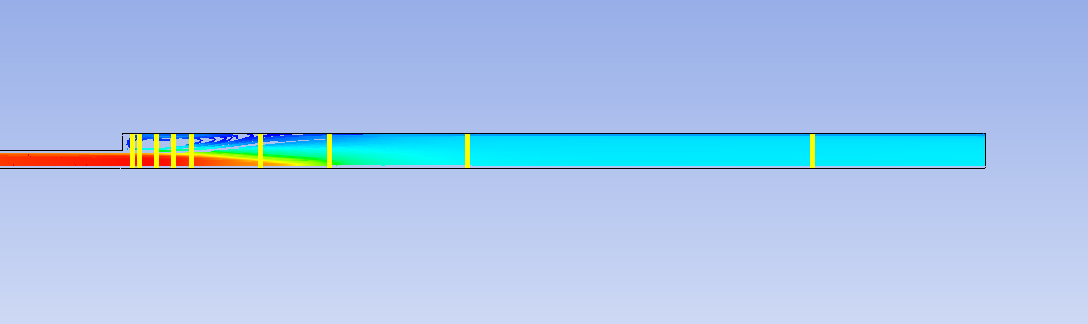
\includegraphics[width=.9\textwidth]{images/task2/task2-1/cross_section_locations.png}
    \caption{Cross Section Locations}
    \label{fig:task2cross}
\end{figure}


\begin{figure}[H]
    \centering
    \begin{subfigure}{.48\textwidth}
    \centering
    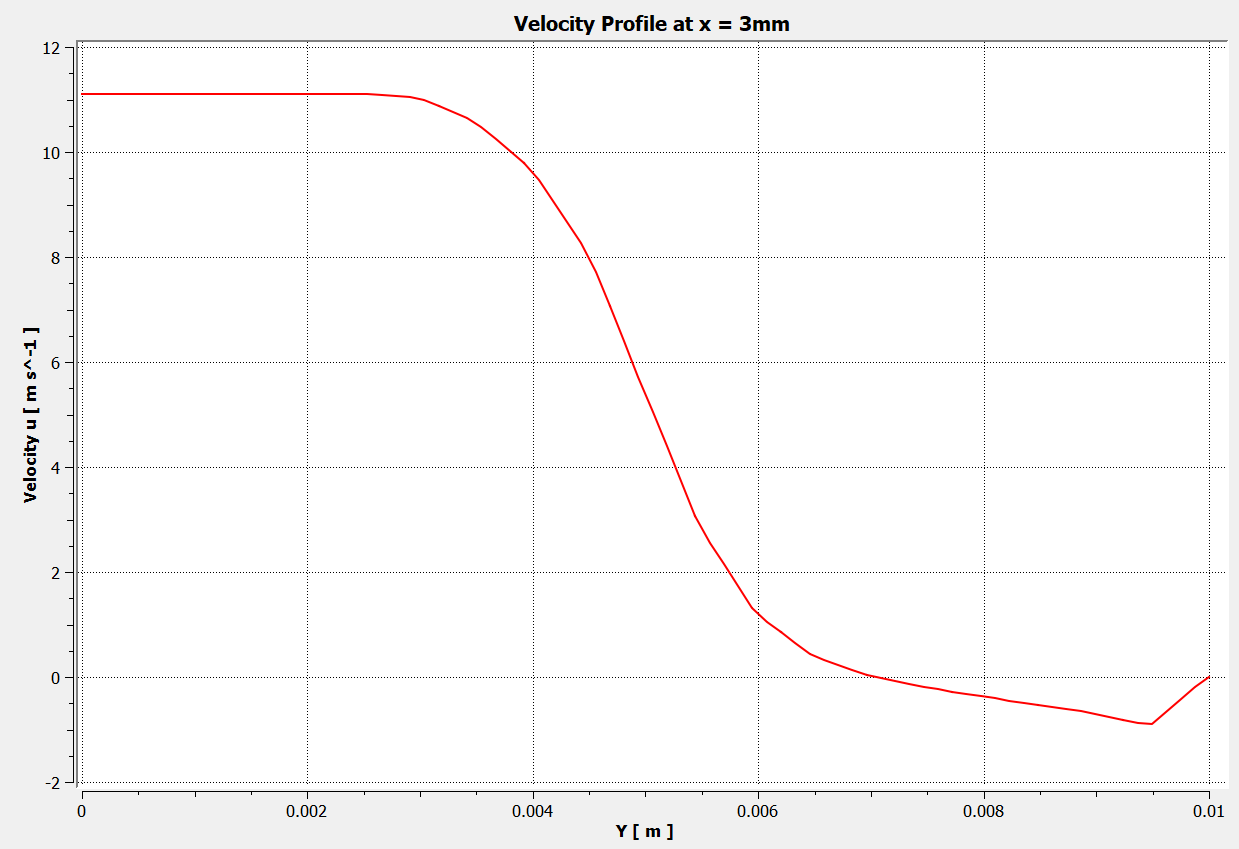
\includegraphics[width=.95\linewidth]{images/task2/task2-1/cs1.png}
    \caption{Velocity profile of $k-\epsilon$ model at x=3mm}
    \end{subfigure}
\hfill
\begin{subfigure}{.48\textwidth}
    \centering
    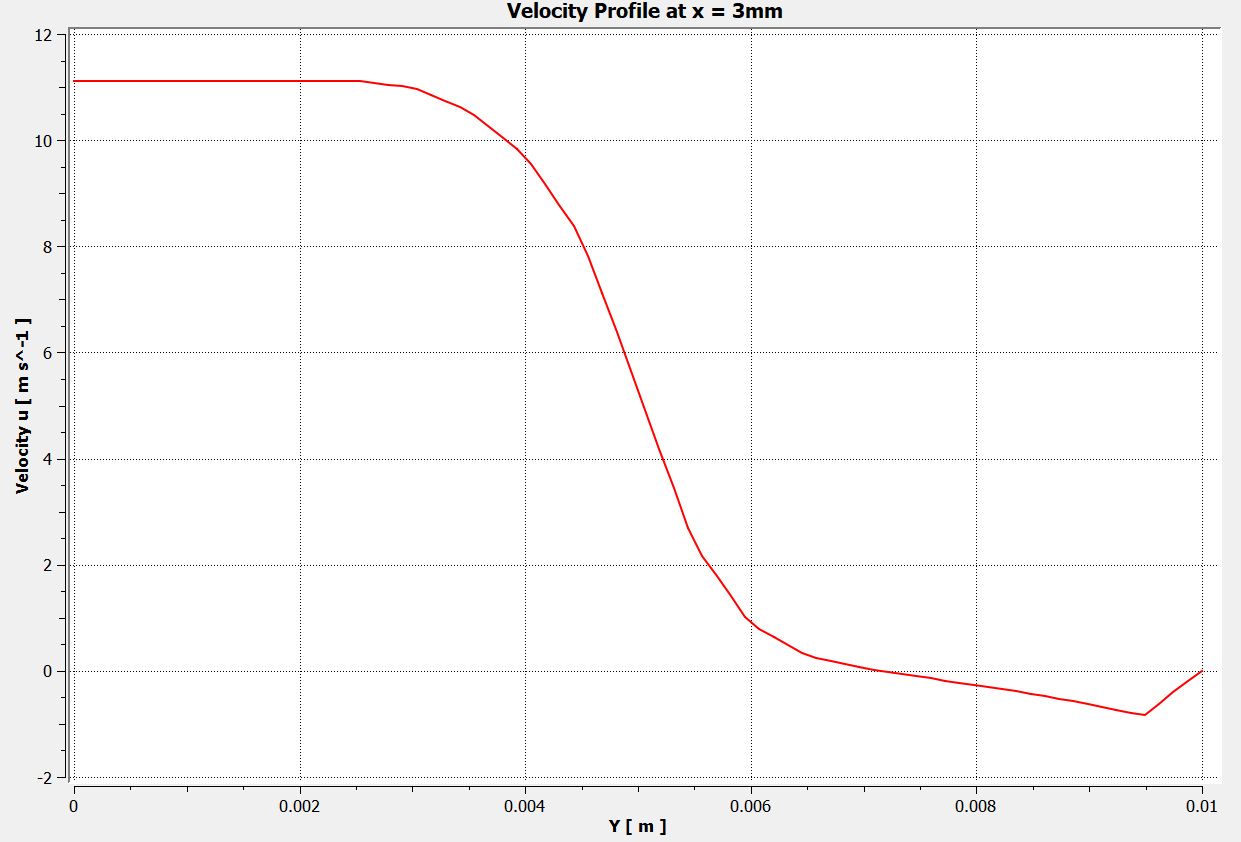
\includegraphics[width=.95\linewidth]{images/task2/task2-2/cs1.png}
    \caption{Velocity profile of $k-\omega$ model at x=3mm}
\end{subfigure}
    ~
    \begin{subfigure}{.48\textwidth}
    \centering
    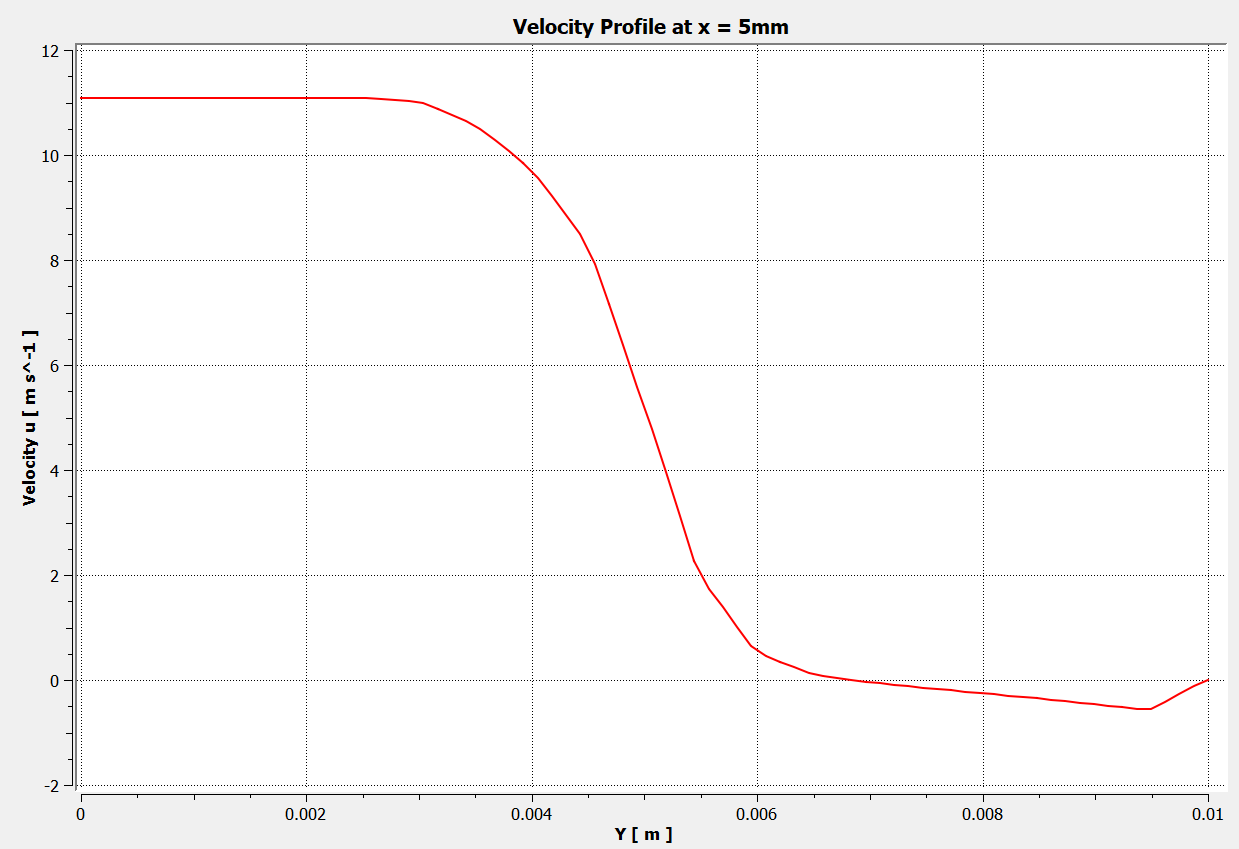
\includegraphics[width=.95\linewidth]{images/task2/task2-1/cs2.png}
    \caption{Velocity profile of $k-\epsilon$ model at x=5mm}
\end{subfigure}
    ~
    \begin{subfigure}{.48\textwidth}
    \centering
    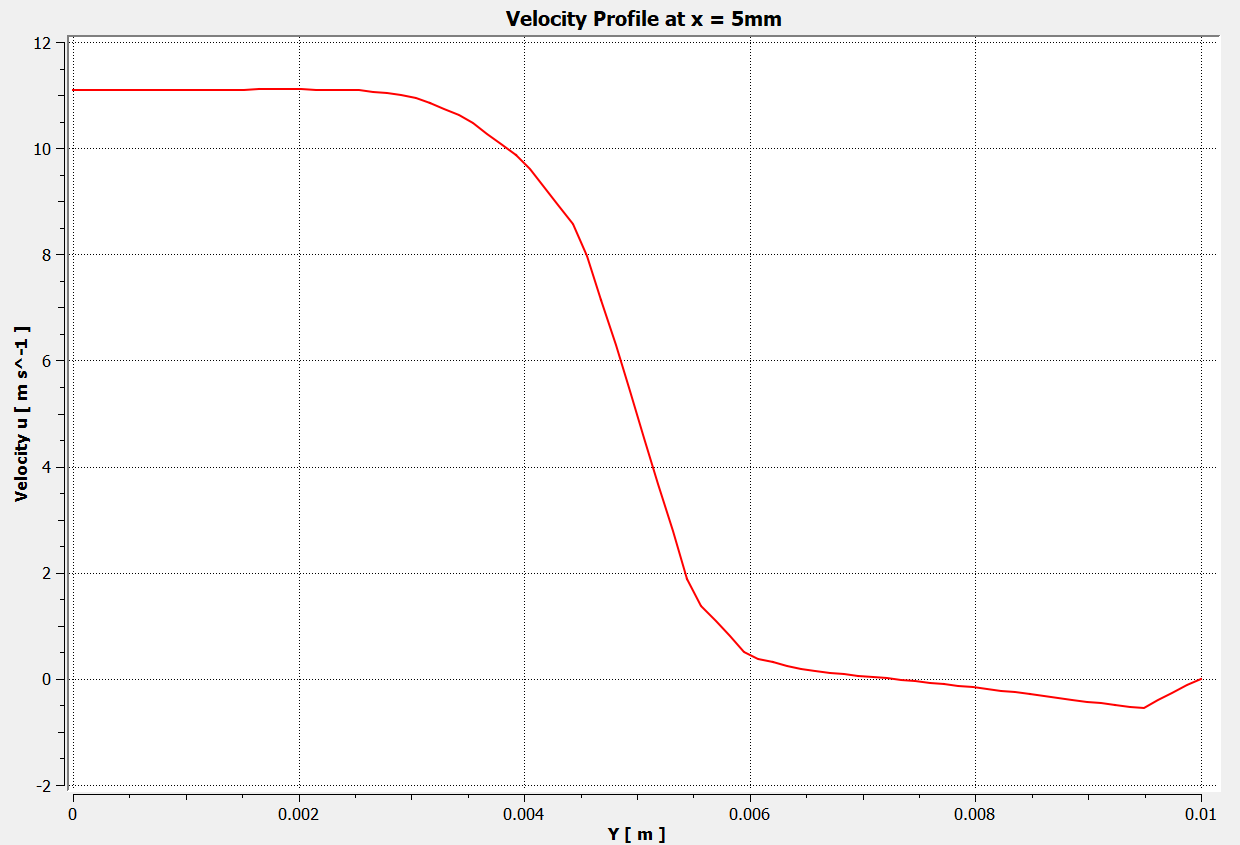
\includegraphics[width=.95\linewidth]{images/task2/task2-2/cs2.png}
    \caption{Velocity profile of $k-\omega$ model at x=5mm}
\end{subfigure}


    ~
    \begin{subfigure}{.48\textwidth}
    \centering
    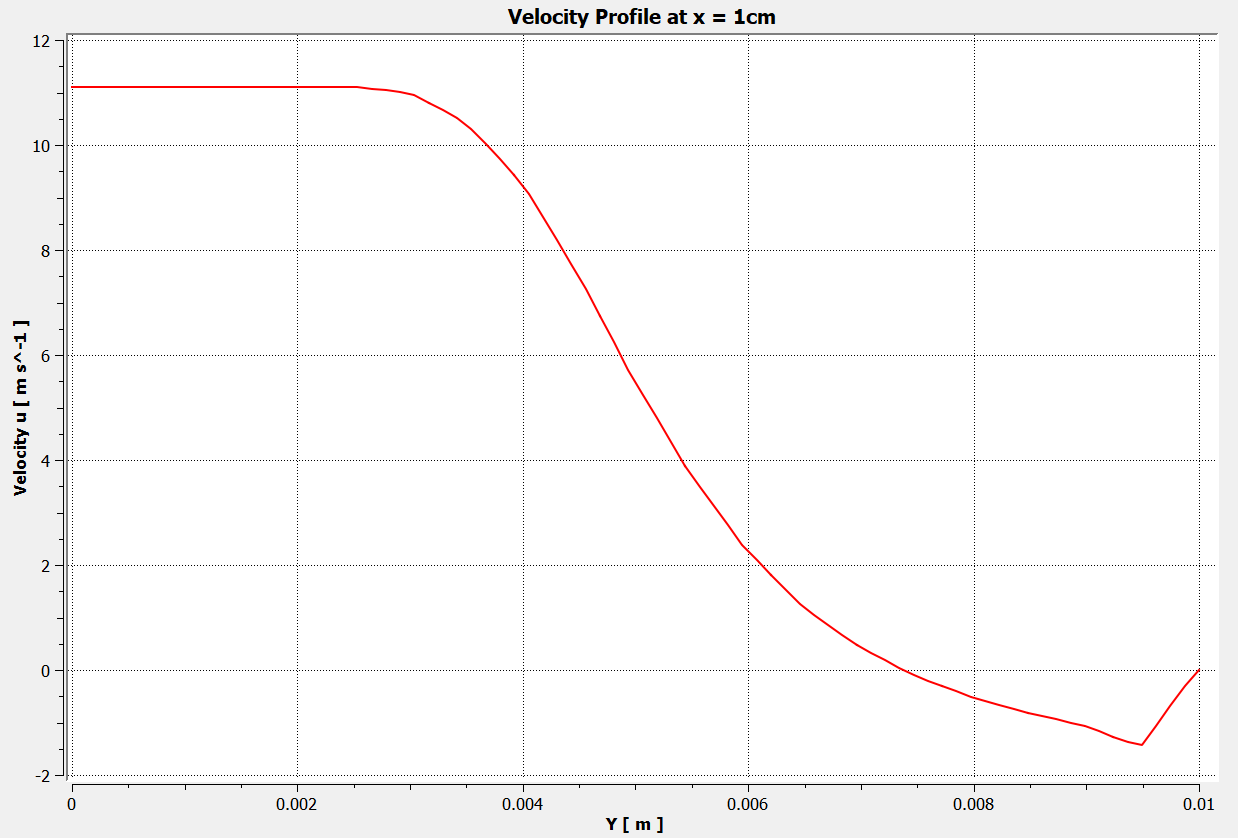
\includegraphics[width=.95\linewidth]{images/task2/task2-1/cs3.png}
    \caption{Velocity profile of $k-\epsilon$ model at x=10mm}
\end{subfigure}
    ~
    \begin{subfigure}{.48\textwidth}
    \centering
    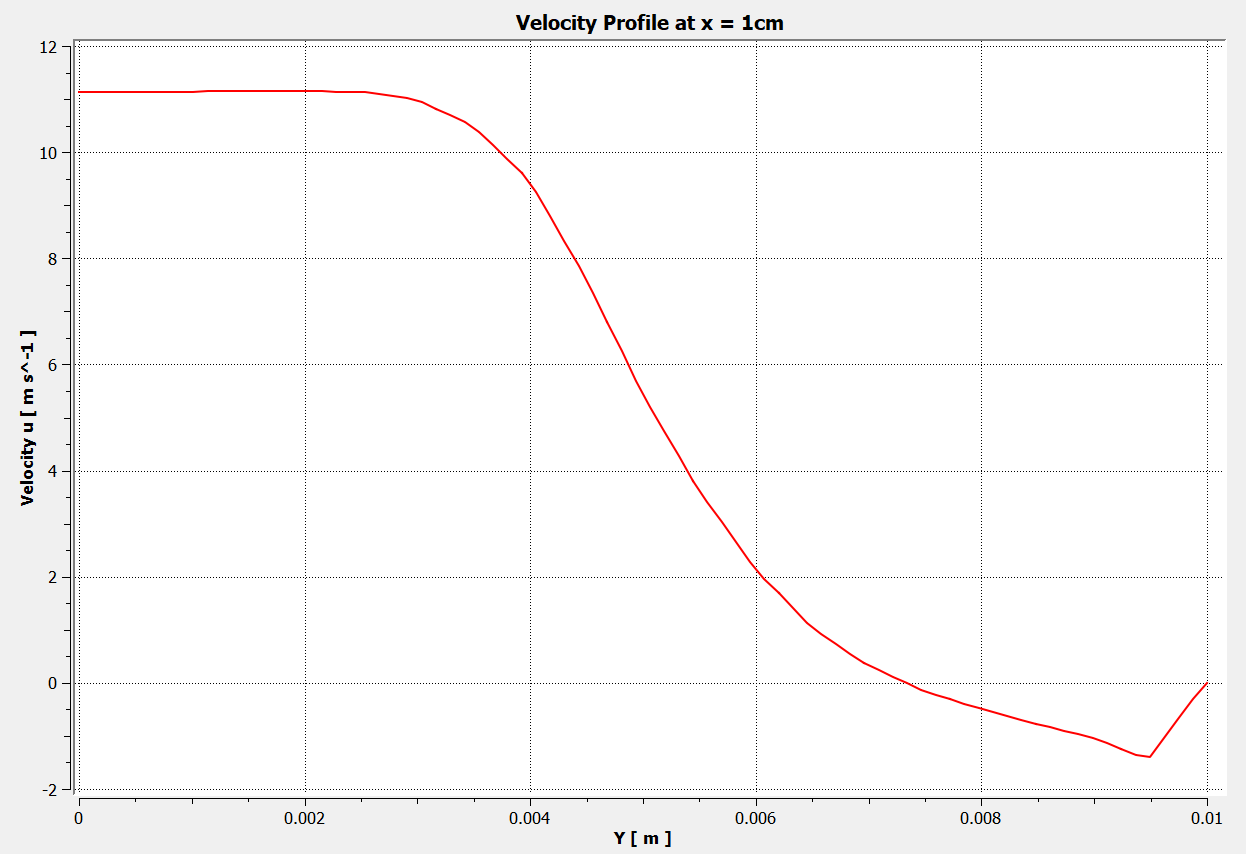
\includegraphics[width=.95\linewidth]{images/task2/task2-2/cs3.png}
    \caption{Velocity profile of $k-\omega$ model at x=10mm}
\end{subfigure}


    ~
    \begin{subfigure}{.48\textwidth}
    \centering
    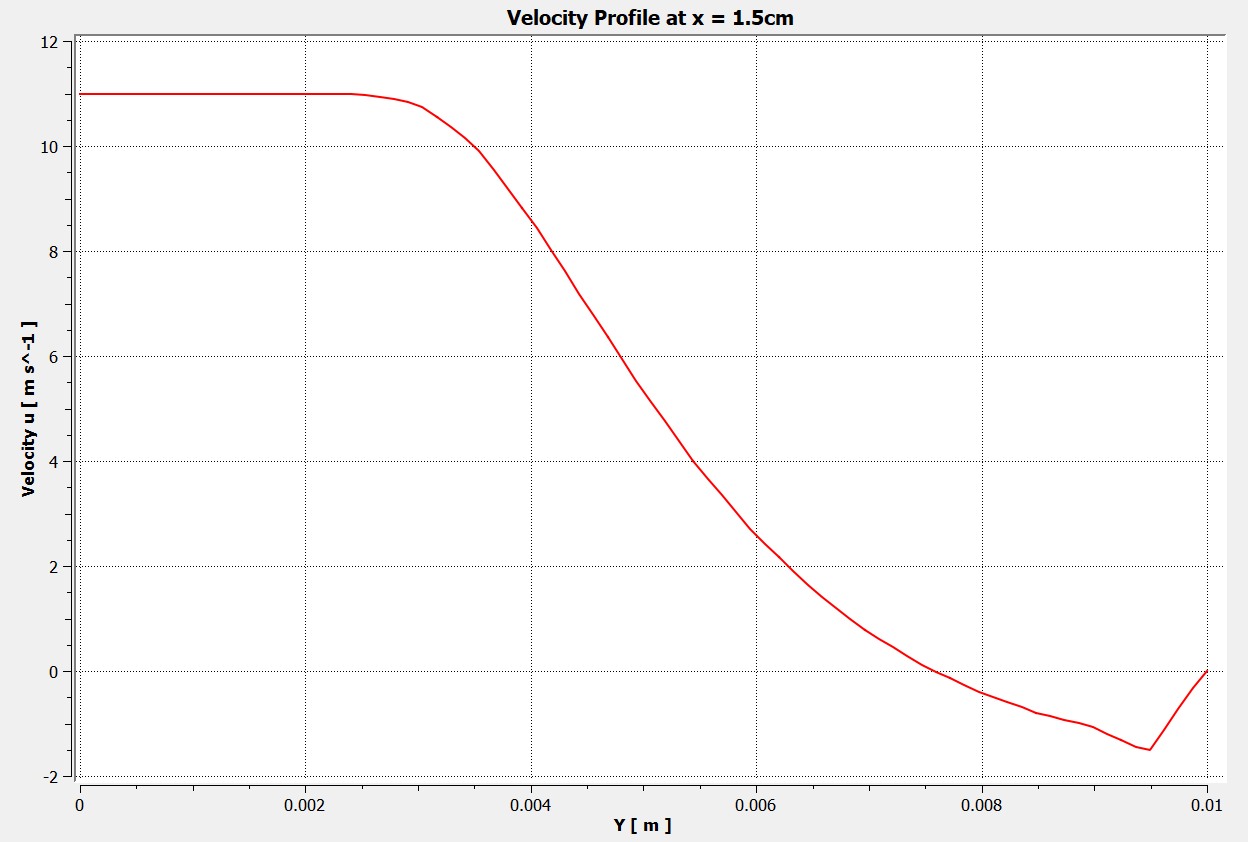
\includegraphics[width=.95\linewidth]{images/task2/task2-1/cs4.png}
    \caption{Velocity profile of $k-\epsilon$ model at x=15mm}
\end{subfigure}
    ~
    \begin{subfigure}{.48\textwidth}
    \centering
    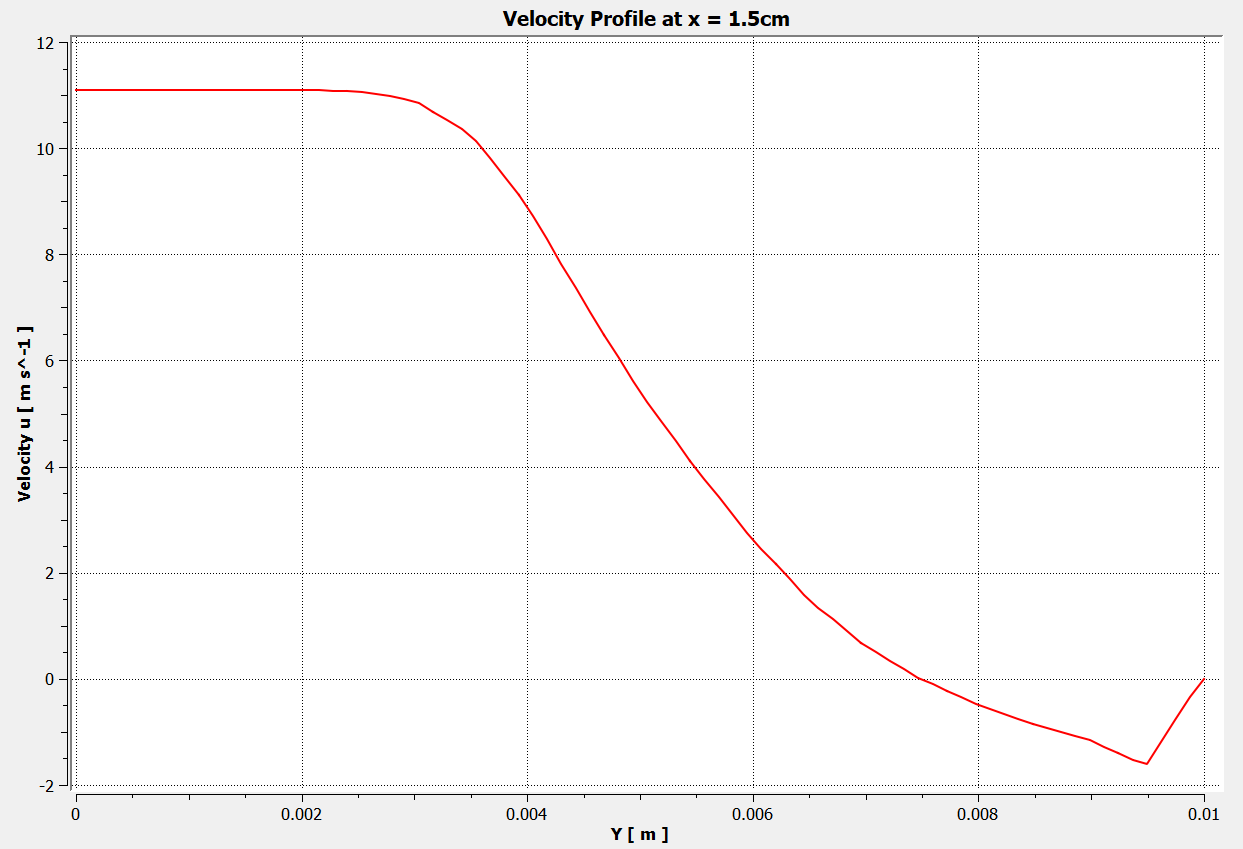
\includegraphics[width=.95\linewidth]{images/task2/task2-2/cs4.png}
    \caption{Velocity profile of $k-\omega$ model at x=15mm}
\end{subfigure}

    \caption{Velocity Profiles}
    \label{fig:task2prof1}
\end{figure}



\begin{figure}[H]
    \centering
     ~
    \begin{subfigure}{.48\textwidth}
    \centering
    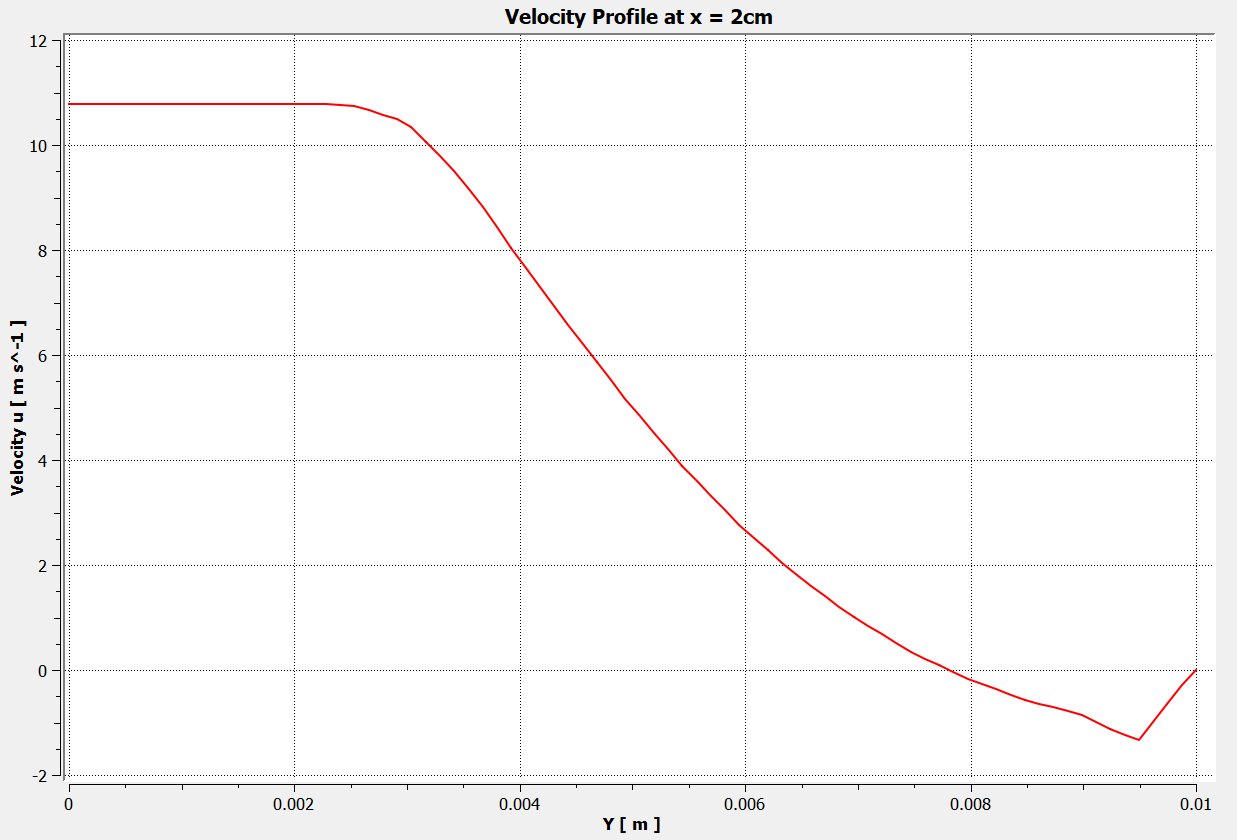
\includegraphics[width=.95\linewidth]{images/task2/task2-1/cs5.png}
    \caption{Velocity profile of $k-\epsilon$ model at x=20mm}
\end{subfigure}
    ~
    \begin{subfigure}{.48\textwidth}
    \centering
    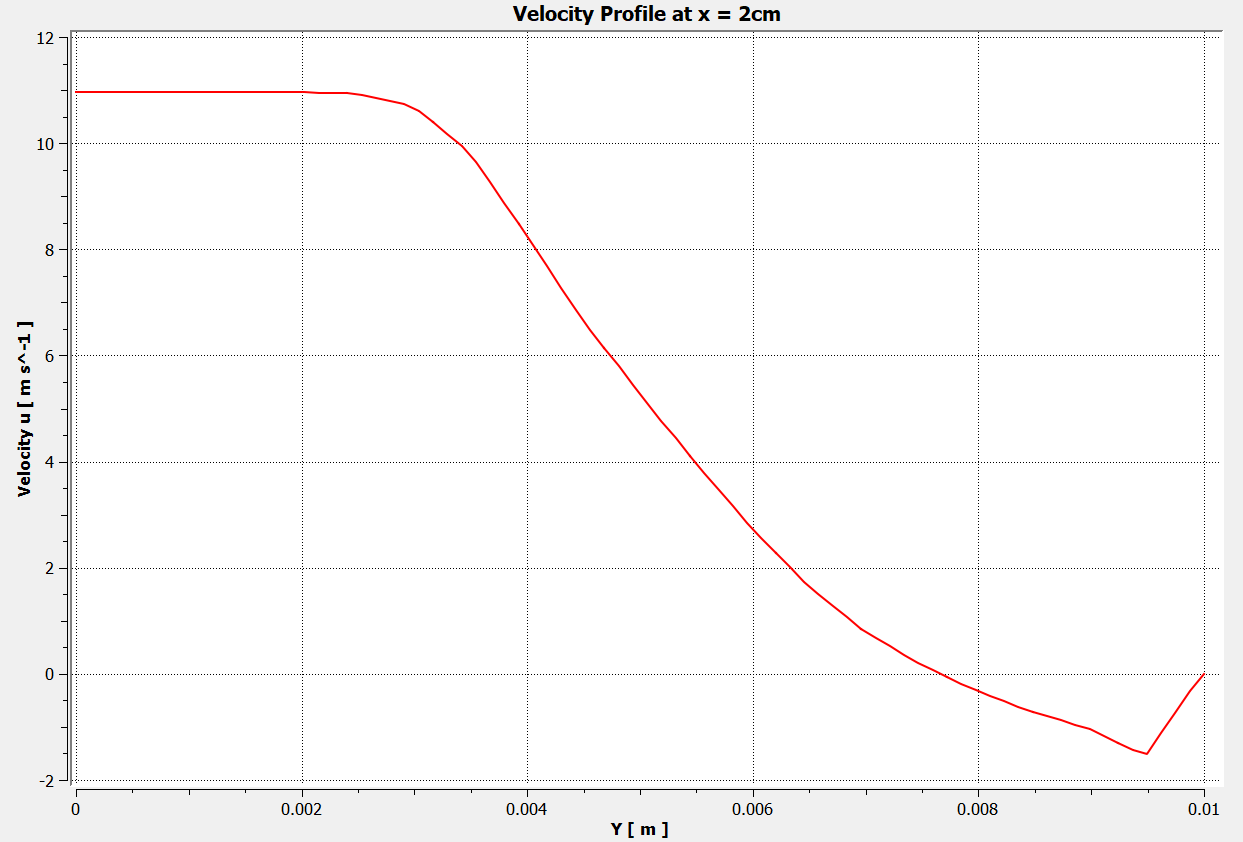
\includegraphics[width=.95\linewidth]{images/task2/task2-2/cs5.png}
    \caption{Velocity profile of $k-\omega$ model at x=20mm}
\end{subfigure}


     ~
    \begin{subfigure}{.48\textwidth}
    \centering
    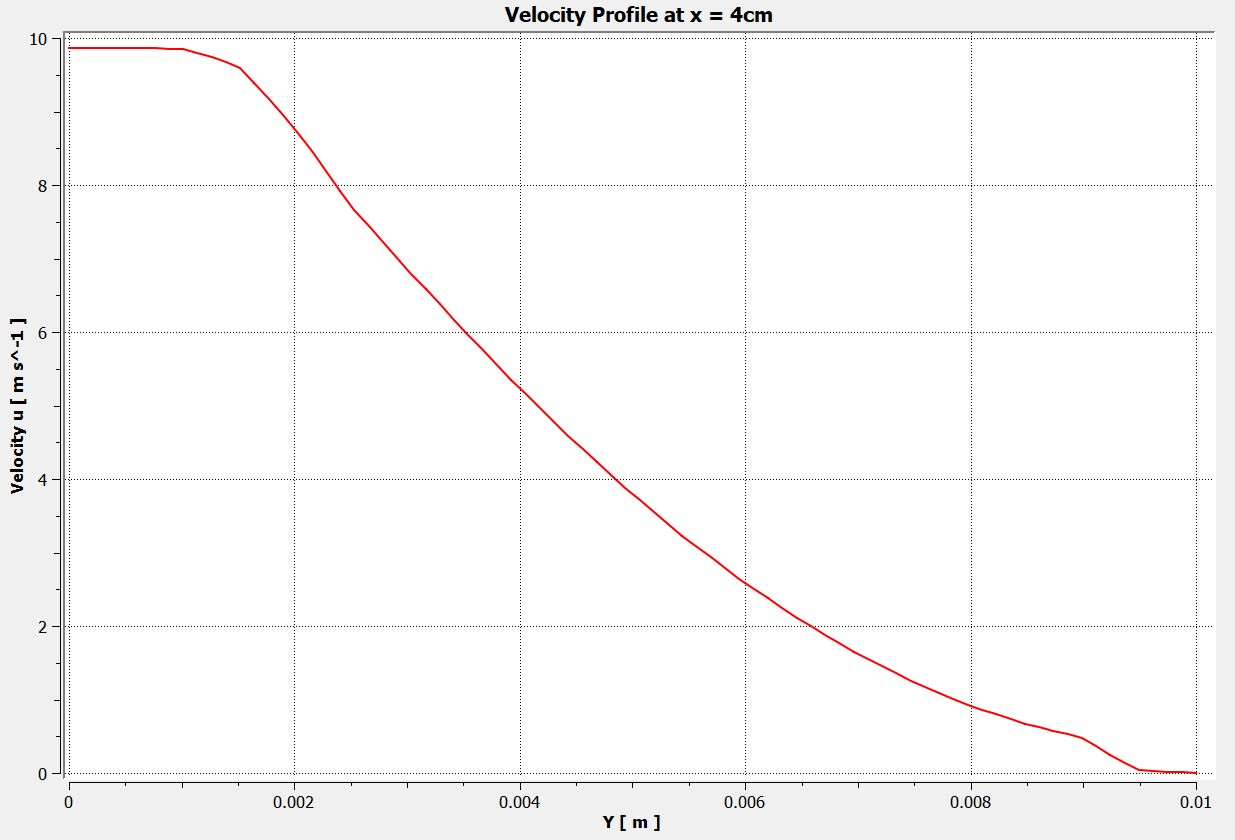
\includegraphics[width=.95\linewidth]{images/task2/task2-1/cs6.png}
    \caption{Velocity profile of $k-\epsilon$ model at x=40mm}
\end{subfigure}
    ~
    \begin{subfigure}{.48\textwidth}
    \centering
    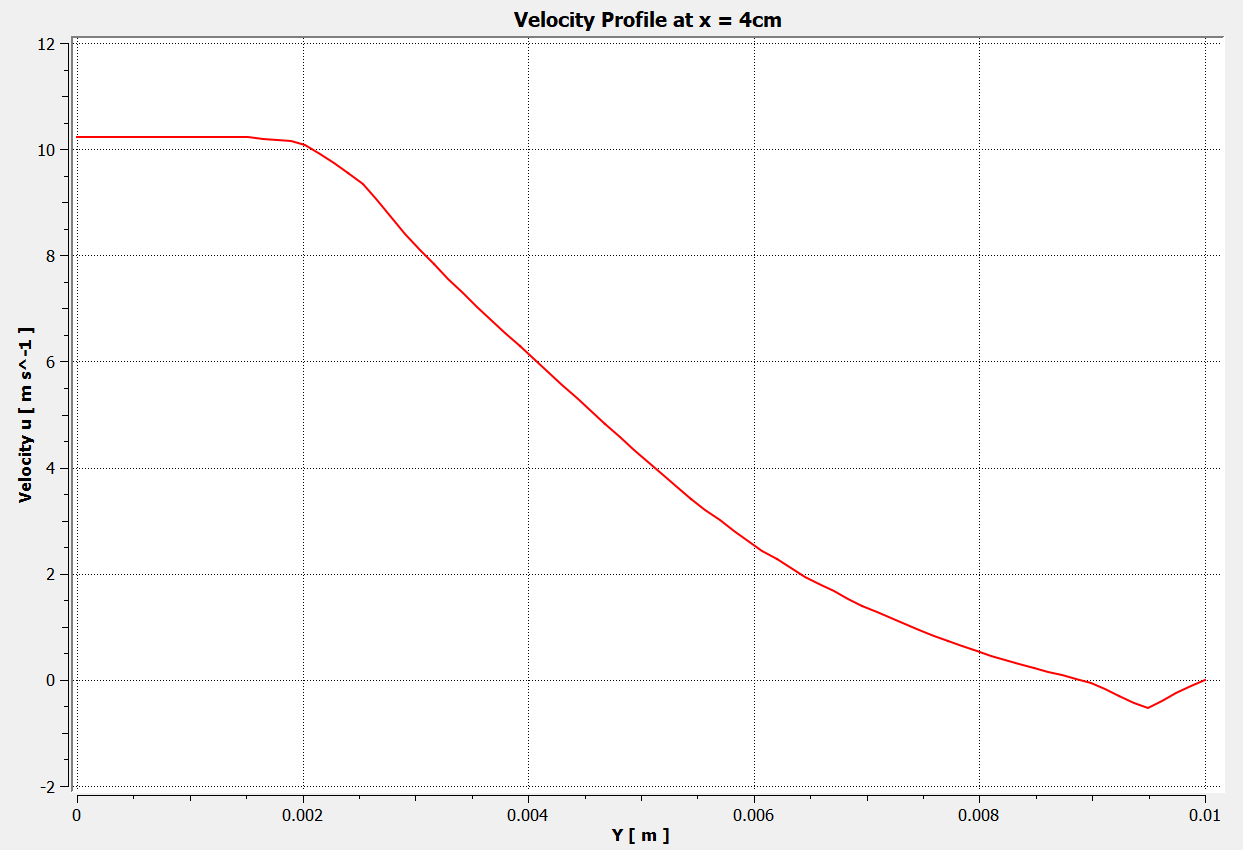
\includegraphics[width=.95\linewidth]{images/task2/task2-2/cs6.png}
    \caption{Velocity profile of $k-\omega$ model at x=40mm}
\end{subfigure}


     ~
    \begin{subfigure}{.48\textwidth}
    \centering
    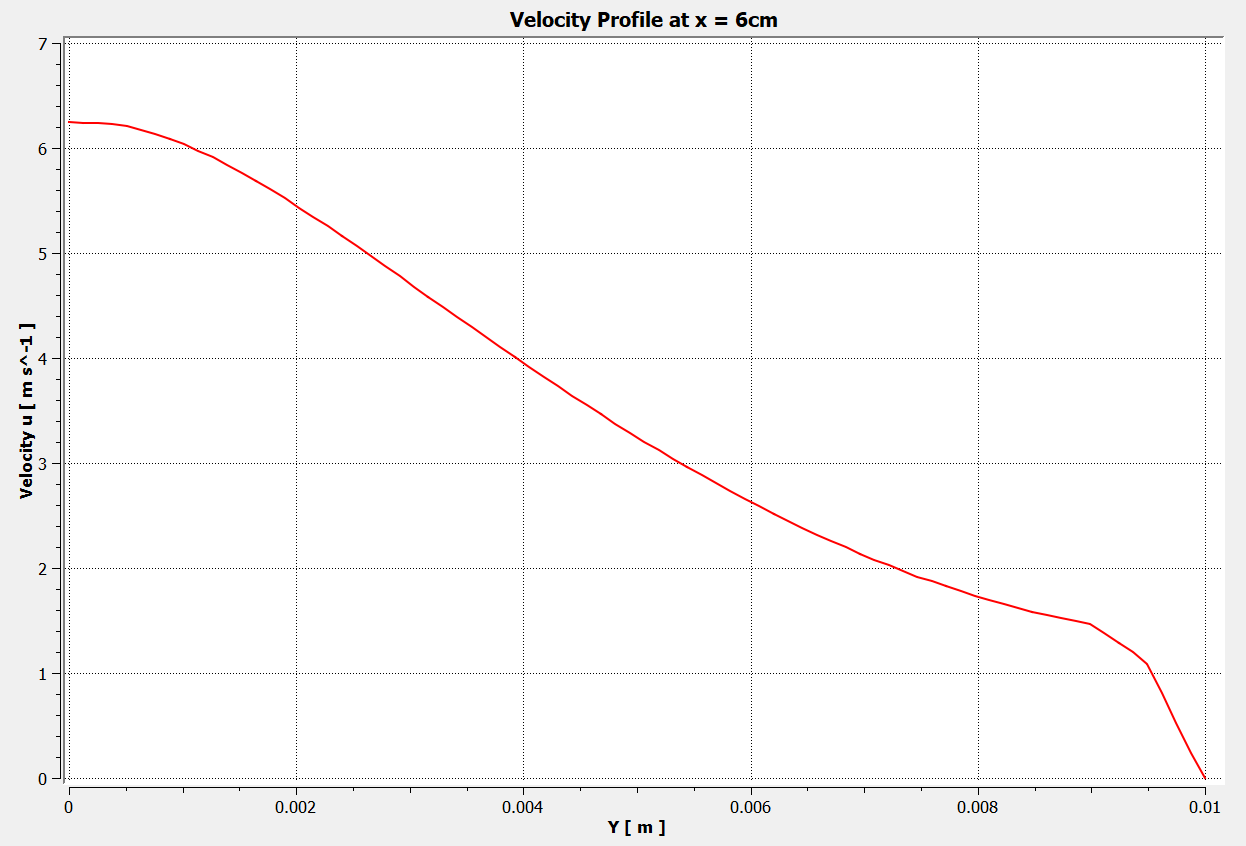
\includegraphics[width=.95\linewidth]{images/task2/task2-1/cs7.png}
    \caption{Velocity profile of $k-\epsilon$ model at x=4=60mm}
\end{subfigure}
    ~
    \begin{subfigure}{.48\textwidth}
    \centering
    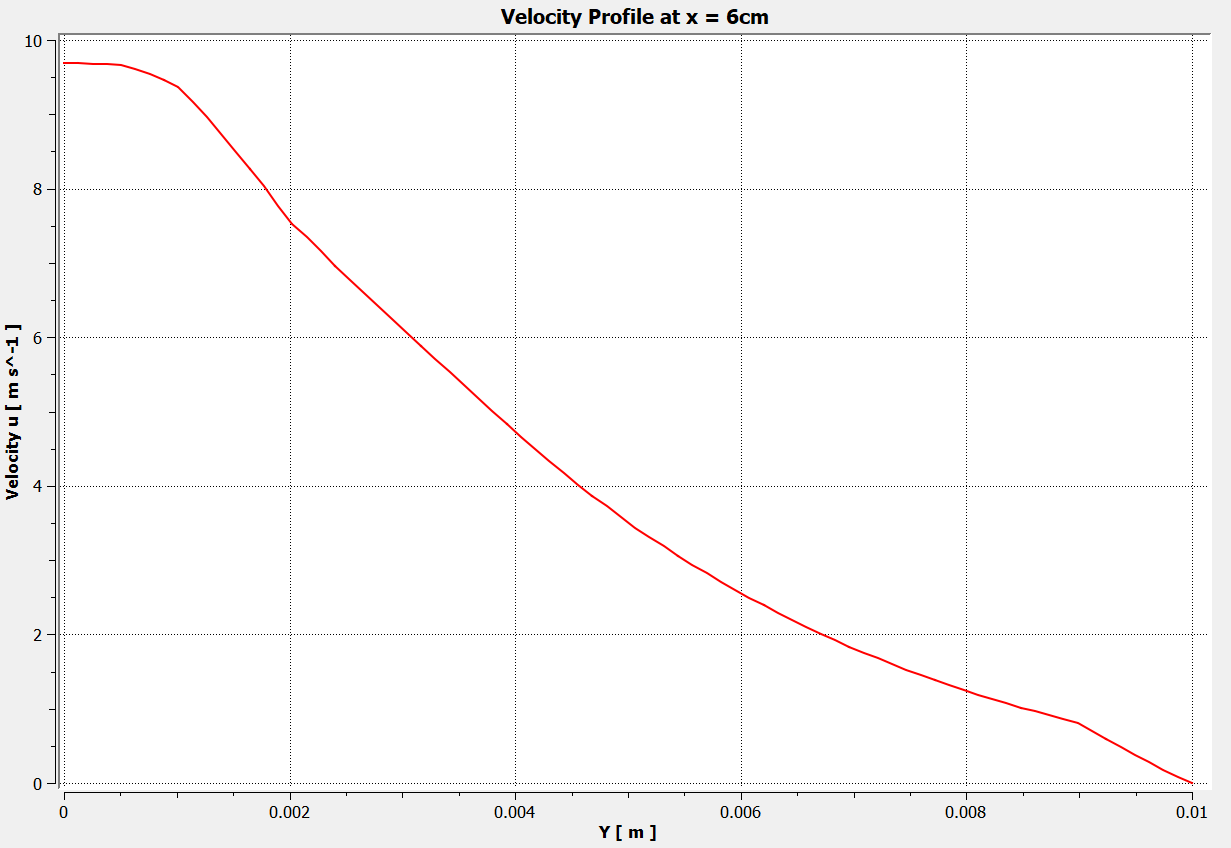
\includegraphics[width=.95\linewidth]{images/task2/task2-2/cs7.png}
    \caption{Velocity profile of $k-\omega$ model at x=4=60mm}
\end{subfigure}



     ~
    \begin{subfigure}{.48\textwidth}
    \centering
    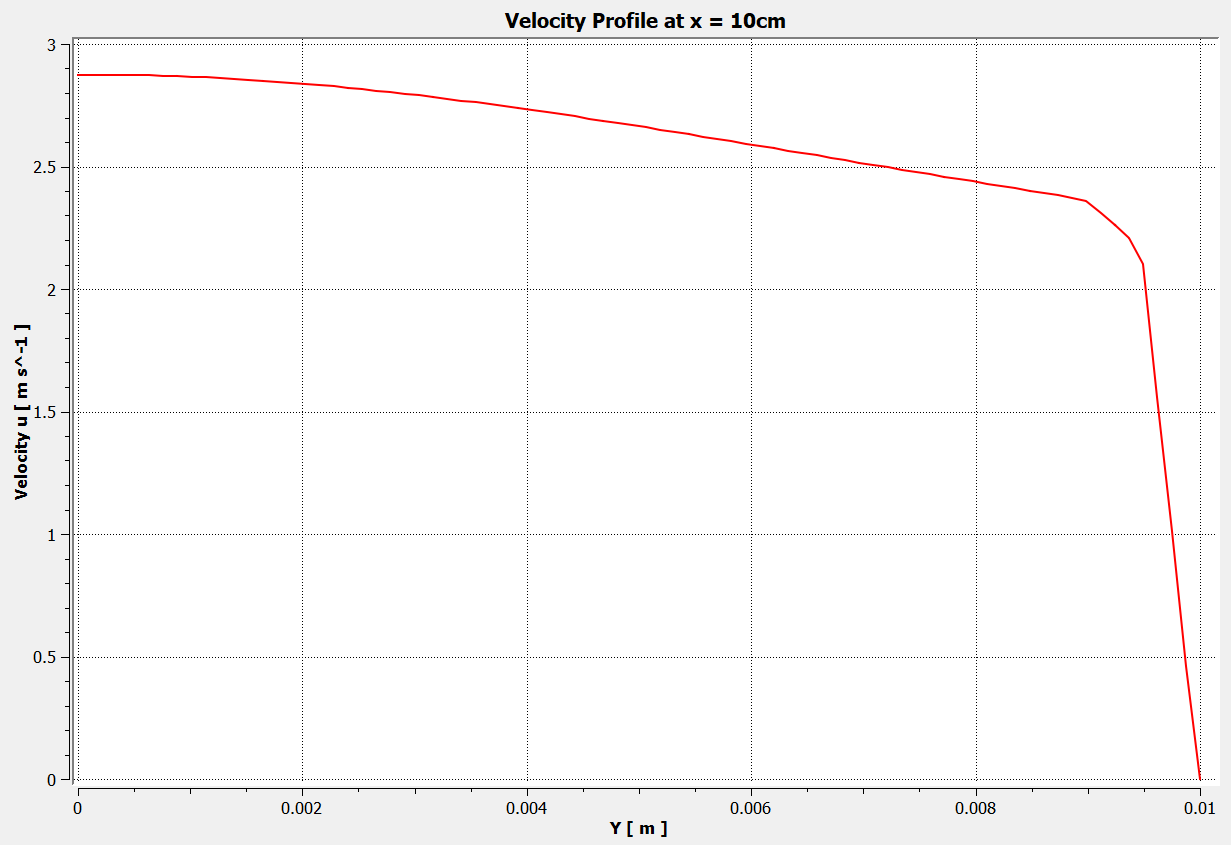
\includegraphics[width=.95\linewidth]{images/task2/task2-1/cs8.png}
    \caption{Velocity profile of $k-\epsilon$ model at x=100mm}
\end{subfigure}
    ~
    \begin{subfigure}{.48\textwidth}
    \centering
    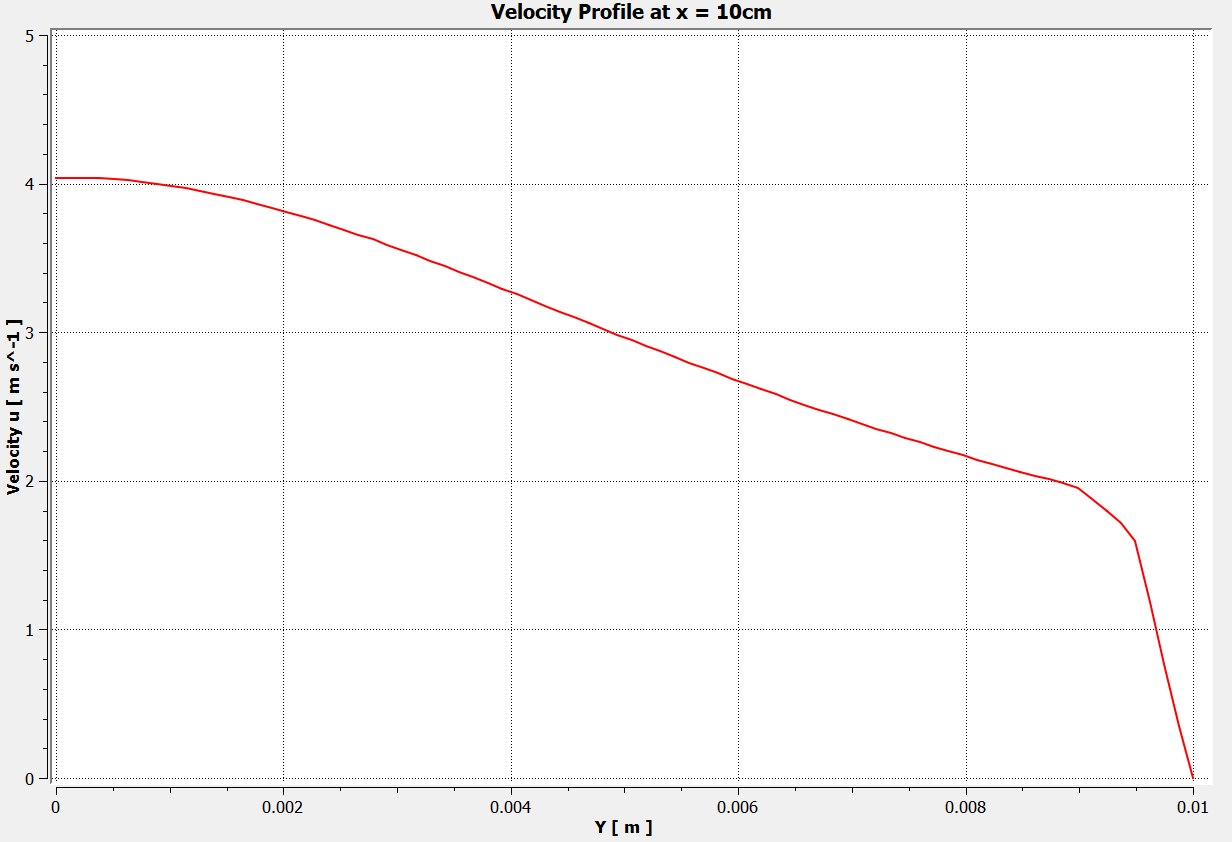
\includegraphics[width=.95\linewidth]{images/task2/task2-2/cs8.png}
    \caption{Velocity profile of $k-\omega$ model at x=100mm}
\end{subfigure}
    
    
    \caption{Velocity Profiles}
    \label{fig:task2prof2}
\end{figure}
\newpage

\subsubsection{Comparison of the Streamlines and Pressure Contours}

\noindent Now that we have seen velocity profiles, streamlines for the two models are the next to be examined. The figure below shows their comparison side-by-side. As guessed from their axial velocity profile, their recirculation zones are different in length. The $k-\omega$ model seems to result in a greater recirculation zone and a higher reattachment length. To support this, their reattachment lengths are shown on Table \ref{tab:task2}


\begin{figure}[H]
    \centering
    \begin{subfigure}{.8\textwidth}
    \centering
    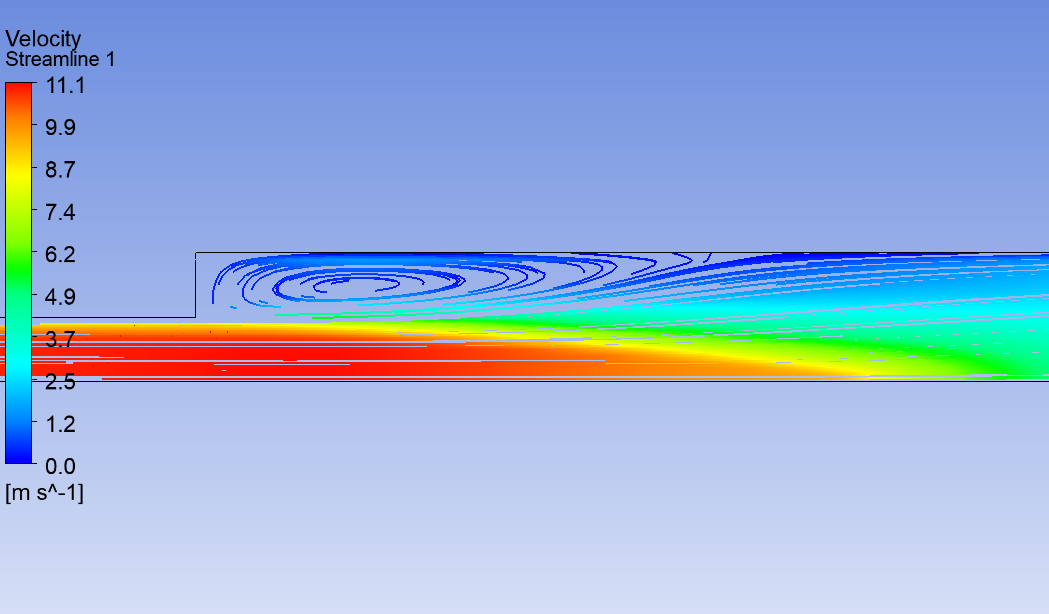
\includegraphics[width=.8\linewidth]{images/task2/task2-1/2-1streamline.png}
    \caption{Streamlines of $k-\epsilon$ model}
    \end{subfigure}
    
\begin{subfigure}{.8\textwidth}
    \centering
    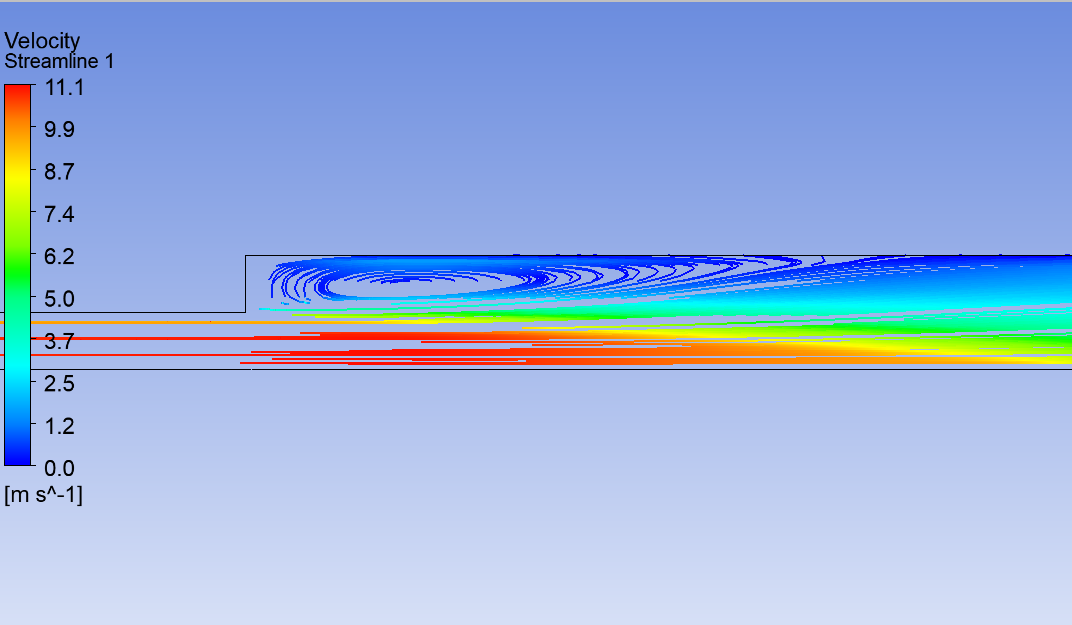
\includegraphics[width=.8\linewidth]{images/task2/task2-2/2-2streamline.png}
    \caption{Streamlines of $k-\omega$ model}
\end{subfigure}
    \caption{Streamlines}
    \label{fig:stream_task2}
\end{figure}


\begin{table}[H]
\centering
\caption{Reattachment Lengths of Models}
\begin{tabular}{c|c}
Model & Reattachment Length (m) \\ \hline
$k-\epsilon$  & 0.039                   \\
$k-\omega$   & 0.051                  
\end{tabular}

\label{tab:task2}
\end{table}

\noindent The last plot that will be of interest to us is the pressure contours in the vicinity of the recirculation zones. Those plots can be seen from Figure \ref{fig:press_task2}.

\begin{figure}[H]
    \centering
    \begin{subfigure}{.85\textwidth}
    \centering
    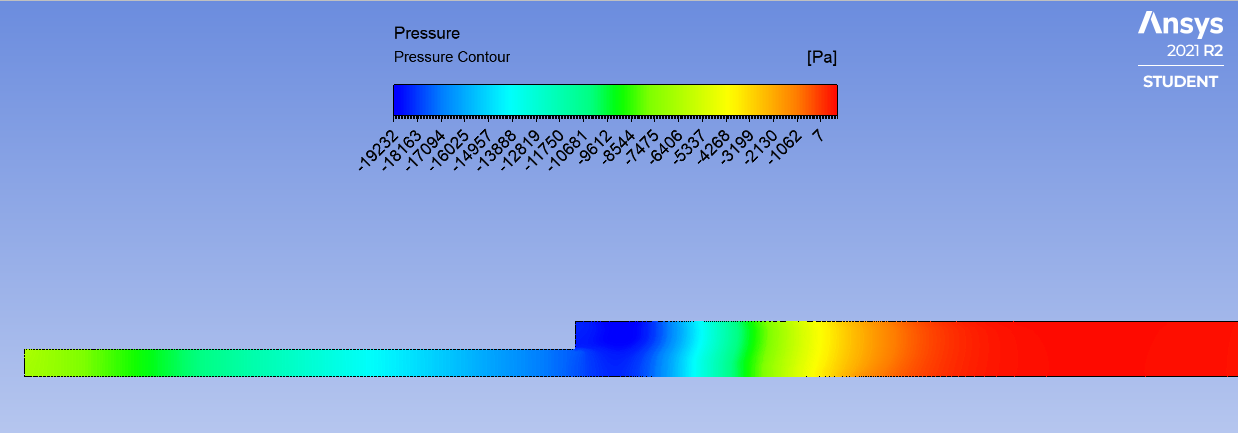
\includegraphics[width=.9\linewidth]{images/task2/task2-1/2-1pressure.png}
    \caption{Pressure contours of $k-\epsilon$ model}
    \end{subfigure}
    
\begin{subfigure}{.85\textwidth}
    \centering
    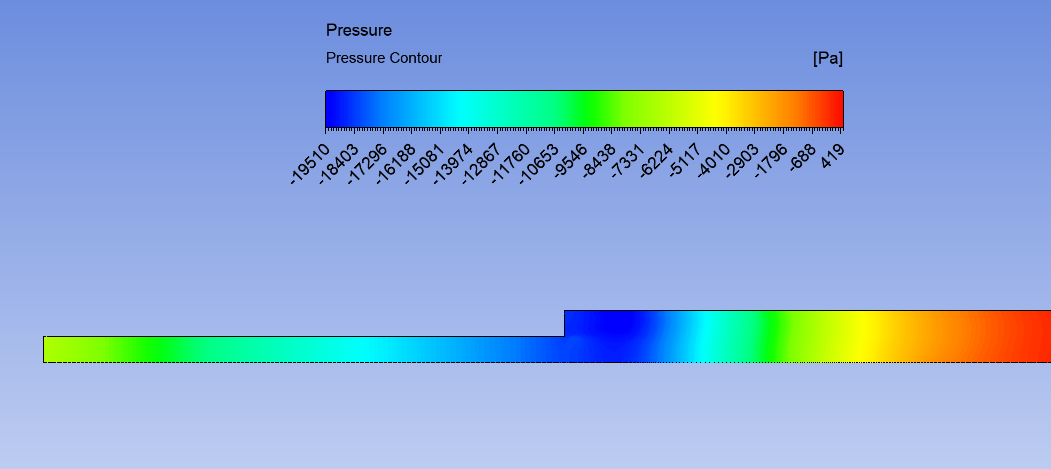
\includegraphics[width=.9\linewidth]{images/task2/task2-2/2-2pressure.png}
    \caption{Pressure contours of $k-\omega$ model}
\end{subfigure}
    \caption{Pressure Contours}
    \label{fig:press_task2}
\end{figure}


\noindent As expected there is a pressure drop induced by the expansion of the pipes. Similar to the streamlines and velocity profiles, the zone in which the pressure drops the most is wider in the $k-\omega$ model, which is in agreement with all the other deductions we have made up to this point. Again caused by turbulences and vortices we observe, the pressure drop return back to normal after some distance from the expansion.